\mysection[black]{3. Lexing and Parsing}


\mysubsection{3.1 Lexing}
\BDEF{Regular Expresssions}{
Define  sets of strings precisely
\begin{tabular}{@{}l l l l@{}}
\toprule
\textbf{Expr.} & \textbf{Desc.} & \textbf{Expr.} & \textbf{Equiv.} \\
\midrule

$\epsilon$ 
& empty 
& $R?$ 
& $(\epsilon \mid R)$ \\

 \texttt{'a'} 
& char 
& \texttt{"foo"} 
& \texttt{'f''o''o'} \\

$R_1 \mid R_2$ 
& $R_1$ or $R_2$ 
& $R^+$ 
& $RR^*$ \\

$R_1 R_2$ 
& $R_2$ follows $R_1$ 
& \texttt{['a'-'z']} 
& $(a \mid \dots \mid z)$ \\

$R^*$ 
& $0 \leq$ reps. 
& \texttt{[\^\,'0'-'9']} 
&  $\mathbf{C}$\texttt{['a'-'z']}  \\
\end{tabular}} 
\textbf{Lexer Generator}: Associate $R_i$ with action $A_i$\\
\textbf{NFA to DFA}: Powerset; collapses $\epsilon$-transitions
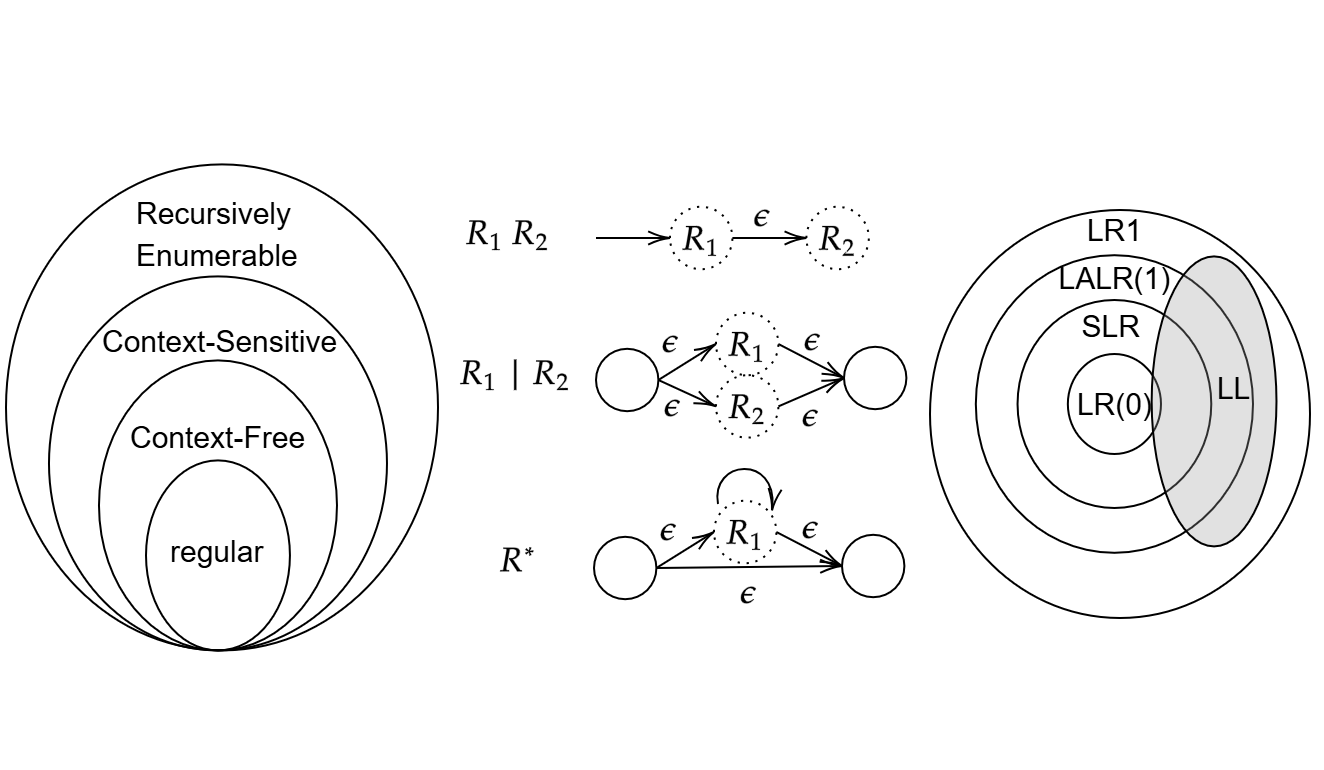
\includegraphics[width=1\linewidth]{images/diagram-lexing-parsing.png}


\mysubsection{3.2 Parsing}
\textbf{Context-Free Grammars (CFG)}: consists of: \textcolor{Aquamarine}{tree-rep}
\begin{itemize}[leftmargin = *,noitemsep]
\item \textbf{Terminals:} lexical token, $\alpha, \beta, (,),..$ ($\epsilon$ isn't) \textcolor{Aquamarine}{leaves}
\item \textbf{NonTerm.:} Syntactic var. $S,T,S',...$ \textcolor{Aquamarine}{internal nodes}
\item \textbf{Production:} Rule $T \mapsto \beta$, which gives $\alpha T \gamma \mapsto \alpha \beta \gamma$
\item \textbf{Start Symbol:} Nonterminal 
 \end{itemize}
 \textbf{LL(k)/LR(k)}: Left-to-right scanning, Right-/Leftmost deriv., k lookahead\\
\textbf{Empty Lang.}: $\not \exists$ finite derivation\\
\textbf{Productiveness}: Rule contains terminal\\
\textbf{Parse-Trees}: Left-/Rightmost derivation yields same tree, order of application not contained\\
\begin{multicols}{2}
\textbf{Left-recursive}\\
$E \mapsto ET$\\ 
LL(1)-incompatible  ($\infty$-rec)\\
LR(1)-compatible

\columnbreak

\textbf{Right-recursive}\\
$E \mapsto TE$\\ 
LL(1)-compatible\\
LR(1)-compatible

\end{multicols}
\textbf{Ambiguity}: Remove my allowing only left-/right-recursion, adding non-terminals\\
\textbf{Precendence}: Determined by how deep (far from the start symbol) an operator is introduced in the grammar. {\color{Aquamarine}$S \to S+S\mid S*S\mid num$ to $S\to T * S \mid T$,$T\to N + T \mid N$,$N\to num $, prec: $+>*$ }\\
\textbf{Mult. Derivations}: An unambiguous CFG can have more than one derivation, all of them correspond to the same abstract syntax tree\\
\textbf{Converting to LL(1)}: $A \mapsto \alpha \beta_1 \mid \alpha \beta_2$ to $A \mapsto \alpha A'$, $A' \mapsto \beta_1$,$A' \mapsto \beta_2$\\



\textbf{Remove Left-Rec./Enforce Right Assoc.}: $A \mapsto A\alpha_1 \mid \ldots  \mid A \alpha_n \mid \beta_1 \mid \ldots \mid \beta_m$ to $A \mapsto \beta_1 A' \mid \ldots  \mid \beta_m A'$, $A' \mapsto \alpha_1 A' \mid \ldots \mid \alpha_n A' \mid \epsilon$ {\color{Aquamarine}$S \to S+S\mid S*S\mid n$ to $S\to n S'$,$S'\to+SS'\mid *SS'\mid \epsilon$} \\




\textbf{Predictive Parsing (PP)}: Given LL(1), lookahead symbol uniquely defines production to apply.\\
\textbf{PP Table}: $\operatorname{nonterminal}\times \operatorname{lookahead} \mapsto \operatorname{production}$\\
\textbf{First}: Pot. start. char $\operatorname{Fst}(\alpha A)=\{\alpha\}$,$\operatorname{Fst}(A\alpha)=\operatorname{Fst}(A)$\\
\textbf{Follow}: terminals that may follow $\$\in \operatorname{Fl}(S)$, $A\mapsto \alpha B a \beta\Rightarrow a \in \operatorname{Fl}(B)$,$A\mapsto \alpha B C \beta \Rightarrow \operatorname{Fst}(C)\setminus \epsilon \subseteq \operatorname{Fl}(B)$. $A\mapsto \alpha B \beta \wedge \epsilon \in \operatorname{Fst}(\beta) \Rightarrow \operatorname{Fl}(A) \subseteq \operatorname{Fl}(B) $ \\
\textbf{Top-down (TD)/Bottom-Up (BU)}: Direction of building parse tree, LL = TD- / LR =BU-parsers \\
\textbf{Shift-Reduce Parser (SRP)}: Algo to impl. LR-pars., $\forall$ LR-parsers are SRP, uses:
\begin{itemize}[leftmargin = *,noitemsep]
\item \textbf{Shift:} Move look-ahead token to stack
\item \textbf{Reduce:} Replace symbols on top of stack with non-terminals
 \end{itemize}
 \textbf{Ex:} Given $S \mapsto S + E \mid E$(1) ,$E \mapsto \operatorname{number}$ (2)
\begin{multicols}{3}
\textbf{Stack}\\
- \\
\texttt{1} \\
\texttt{E} \\
\texttt{S} \\

\columnbreak
\textbf{Input}\\
\texttt{1 + 2} \\
\texttt{ + 2} \\
\texttt{ + 2} \\
\texttt{ + 2}\\
\columnbreak
\textbf{Action}\\
shift \texttt{1} \\
reduce (2) \\
reduce (1) \\
shift  \texttt{+}


\end{multicols}

\textbf{LR(0)}: No look-ahead, state given by $A\mapsto \alpha.\beta$, $\alpha$ consumed, $\beta$ potential upcoming input, tracks corrent state, if $\beta = \epsilon$, eligible for reduction\\
\textbf{Action Selection Problem}: Both shift and reduce may be possible, not clear what to take\\
\textbf{LR(0) to DFA}:   \textcolor{Aquamarine}{Example} ${\color{Aquamarine}S\mapsto (L) \mid id, L\to S \mid L,S}$
\begin{enumerate}[leftmargin = *,noitemsep]
\item Add $S' \mapsto S\$$ to grammar
\item Add Initial item with empty lookahead ${\color{Aquamarine}S'\mapsto .S \$, \{\}}$
\item If state contains dot before nonterminal, compute closure of state with lookahead ${\color{Aquamarine}S'\mapsto .S \$,S\mapsto . (L),\{\$\};S\mapsto . \operatorname{id},\{\$\}}$   
\item Add transition for each non-/terminal after the dot.  , the new state moves the dot  \textcolor{Aquamarine}{Transitions: ${\color{Aquamarine}\operatorname{id},(,S}$}, \textcolor{Aquamarine}{Added States: ${\color{Aquamarine}S'\mapsto S. \$,S\mapsto (.L),S\mapsto  \operatorname{id}.}$   }
\item For each new state start with step 3. again
\end{enumerate}


\textbf{Parsing-Table (LR0)}: Possible actions, use to determine parsing
$$( s, X) \mapsto
\begin{cases}
\text{shift } + \text{goto } s' & X \in \operatorname{terminal} \\
\text{goto } s' & X \in \operatorname{non-terminal} \\
\text{reduce } A \to \alpha
\end{cases}
$$
\textbf{Limitations}: Only works if reduce actions are unique, otherwise shift/reduce or reduce/reduce conflicts\\
\textbf{LR(1)}: Item is LR(0) item with look-ahead\\
\textbf{LR(1) closure}: \\$\forall [A \rightarrow \alpha \cdot B \beta, t] \text{ in } S;\forall \text{production } B \rightarrow \gamma \text{ in } G;
\forall \text{ token } b \text{ in } \text{FIRST}(\beta t); \text{Add } [B \rightarrow \cdot \gamma, b] \text{ to } S$\\


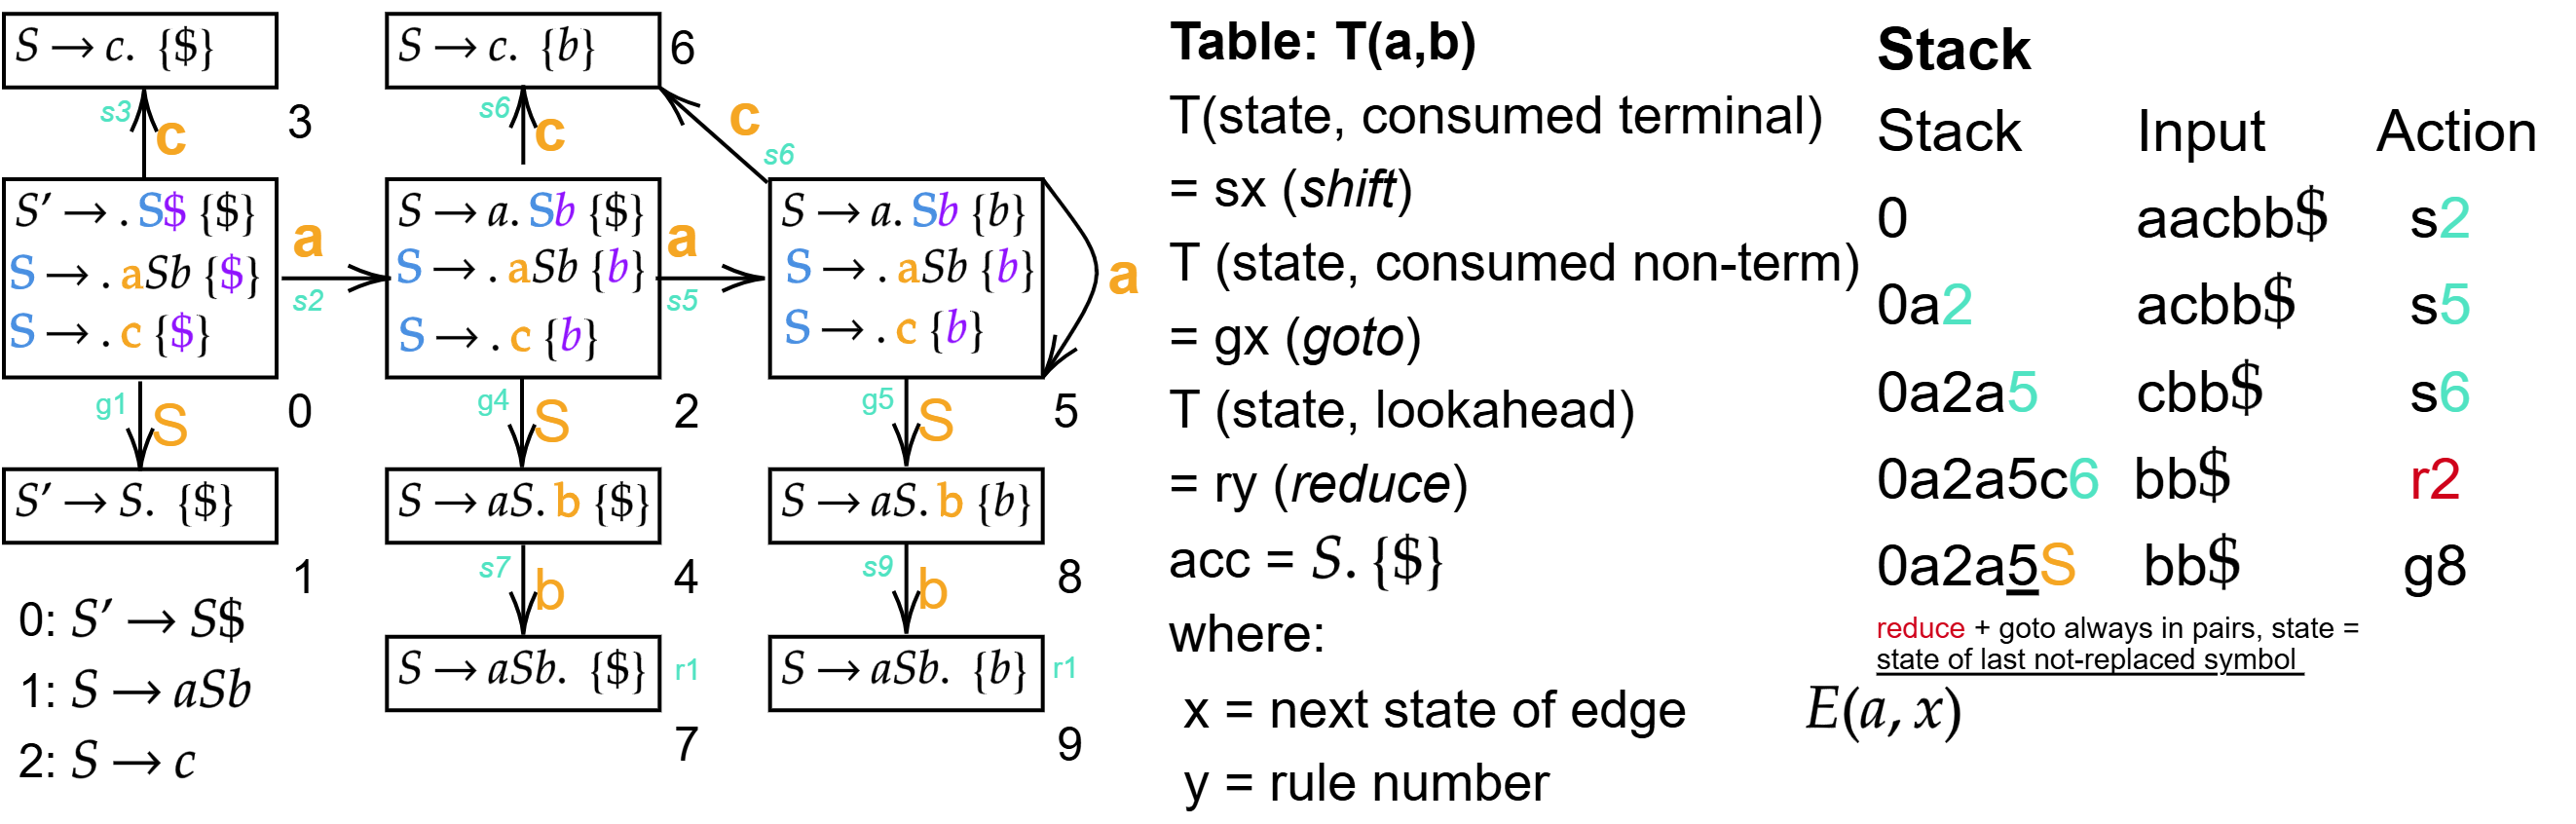
\includegraphics[width=1\linewidth]{images/parsing-table.png}


\textbf{LALR(1)}: Merging LR(1) states that have the same LR(0) core and combine look-ahead, factor 10 fewer states, may only introduce reduce/reduce conflicts i.e. $[X \mapsto a. , a],[X \mapsto a. , b] \Rightarrow [X \mapsto a. , a/b]$\\
\textbf{SLR}: Simple LR, uses follow     \\
\textbf{GLF}: Generalized LR, computes all parses for input and disambiguate based on context \\


